\chapter{Desarrollo}
\label{develop}

El desarrollo del emulador se estructura en diversas fases que abordan los principales componentes de la consola, comenzando por la CPU, continuando con la gestión de gráficos (GPU/PPU) y memoria (RAM/ROM), y concluyendo con la implementación de las interfaces de entrada y salida (I/O). Cada uno de estos módulos es fundamental para asegurar una emulación fiel al hardware original, por lo que se prestará especial atención a la precisión y al rendimiento.
\\\\
La primera fase se centrará en la implementación de la CPU, que es responsable de ejecutar las instrucciones del juego. Cada paso del desarrollo irá acompañado de pruebas y validaciones para garantizar que el emulador reproduzca el comportamiento de la consola original de manera eficiente. Esto último se conseguirá mediante la implementación de pruebas unitarias que verifiquen el correcto comportamiento de los opcodes.

\section{Módulos / Estructura del Proyecto}

El emulador que se va a implementar constará de distintos módulos, cada uno con una función específica y clara, lo que facilitará tanto su comprensión como el desarrollo de cada uno de los aspectos del emulador. A continuación, se describen brevemente los módulos principales del proyecto:

\begin{itemize} 
    \item \textbf{Emulator}: Este módulo centraliza la gestión de los otros componentes, coordinando su interacción y asegurando que el ciclo de emulación se ejecute correctamente. Controla el flujo general del programa.
    \item \textbf{CPU}: Responsable de la ejecución de las instrucciones. Se encarga de la implementación del conjunto de instrucciones de la Game Boy y la simulación de los registros, el Program Counter (PC), el Stack Pointer (SP) y las operaciones con la ALU.
    \item \textbf{Memory}: Gestiona el acceso a la memoria principal del sistema. Proporciona una interfaz para leer y escribir datos en las distintas áreas de la memoria del emulador, incluyendo ROM, RAM y áreas de E/S.
    \item \textbf{ROM}: Módulo encargado de cargar y gestionar la memoria ROM, que contiene el código del juego o programa a emular. Lee los datos directamente desde el archivo del juego y los pone a disposición del emulador.
    \item \textbf{RAM}: Controla la memoria de acceso aleatorio del sistema, donde se almacenan temporalmente datos durante la ejecución del programa. Es volátil y se borra cada vez que se reinicia el sistema.
    \item \textbf{PPU (Pixel Processing Unit)}: Se encarga de la representación gráfica. Simula la unidad de procesamiento de píxeles de la consola, manejando la creación y renderización de sprites y fondos en pantalla.
    \item \textbf{Timer}: Simula los temporizadores de la consola, necesarios para sincronizar eventos y gestionar interrupciones relacionadas con el tiempo, como el reloj del sistema y los temporizadores de la CPU.
    \item \textbf{Interrupt}: Maneja las interrupciones generadas por los eventos del sistema, como teclas presionadas, cambios en el PPU o eventos de temporización. Se encarga de priorizarlas y derivarlas a las funciones correspondientes.
    \item \textbf{IO (Input/Output)}: Administra las interacciones de entrada y salida, como las pulsaciones de los botones del usuario y la comunicación con dispositivos externos.
    \item \textbf{DMA}: Permite la transferencia de datos entre la memoria de vídeo y la memoria principal sin la intervención del CPU. Facilita la copia eficiente de gráficos y sprites, optimizando el rendimiento al liberar al CPU para otras tareas durante las transferencias de datos.
    \item \textbf{FifoFetcher}: Gestiona la recuperación de datos de píxeles de la memoria de video, utilizando una estructura FIFO para almacenar temporalmente la información de tiles y atributos. Su función principal es asegurar una carga eficiente de píxeles para la representación gráfica en pantalla.
    \item \textbf{Audio}: Genera y manipula sonidos en la Game Boy, gestionando canales de audio como ondas de pulso y ruido. Controla la frecuencia, duración y mezcla de los sonidos.
\end{itemize}

\section{CPU}

El desarrollo comienza con la implementación de la Unidad Central de Procesamiento. Debido a su papel fundamental en la correcta reproducción del funcionamiento del sistema, esta etapa se centra en implementar todas las instrucciones para asegurar que el emulador pueda procesar cada byte de información con precisión.

\subsection{Registros}
Para definirlos en nuestro programa, utilizaremos el tipo Byte o UByte de Kotlin. En mi caso por desconocimiento del segundo tipo, comencé a programarlo con Byte. La diferencia entre ambos es que Byte utiliza el rango de [-128:128] y UByte el de [0:255] (igual que la GB). Podemos hacer uso de cualquiera de los dos mientras tengamos en mente que, si el primero lo convertimos a Integer, será un valor distinto al original. En cuanto a PC y SP, optaremos por utilizar Integers, ya que son valores de 2 bytes y siempre contienen una dirección de memoria.

\begin{lstlisting}[language=Kotlin, caption={Declaración de Registros}, label={code:kotlinregistros}]
    var A: Byte = 0
    var F: Byte = 0             // Contains the 4 flags (11110000 -> ZNHC0000)
    var B: Byte = 0
    var C: Byte = 0
    var D: Byte = 0
    var E: Byte = 0
    var H: Byte = 0
    var L: Byte = 0

    // 16 bits registers
    var SP: Int = 0xFFFE        // Stack Pointer
    var PC: Int = 0             // Program Counter
\end{lstlisting}

Para operar con ellos a nivel de byte, deberemos pasarlos a Integer, aplicarles una operación AND con el valor 0xFF (para eliminar el signo en caso de se utilice el tipo Byte originalmente), se ejecutarían las operaciones necesarias y al resultado se le aplicaría el mismo AND, para justo después volver a convertirlo a Byte:

\begin{lstlisting}[language=Kotlin, caption={Ejemplo de Opcode}, label={code:kotlinexample}]
    fun add_a_c(): Int{
        val intA = A.toInt() and 0xFF // Conversión de Byte a Integer sin signo -> A
        val intC = C.toInt() and 0xFF // Conversión de Byte a Integer sin signo -> C
        val result = intA + intC // Se suman ambos valores (ADD)
        A = (result and 0xFF).toByte() // Al resultado se le quita el signo por precaución y se convierte a Byte

        updateAddOperationFlags(intA, intC, result) // Se actualizan los Flags correspondientes

        return CYCLES_4 // Devolvemos los ciclos que la CPU debe tardar en ejecutar la instrucción
    }
\end{lstlisting}

Para la actualización de los flags, se implementarán funciones específicas que gestionarán su estado de manera adecuada. Adicionalmente, se declararán constantes que facilitarán la identificación del estado de cada flag en cualquier momento. Estas constantes corresponden a los bits asociados con un valor de 1 en formato hexadecimal (por ejemplo, 0x80 corresponde a 0b10000000).

\begin{lstlisting}[language=Kotlin, caption={Actualización de Flags}, label={code:kotlinflags}]

    // Flags --> Booleans
    const val FLAG_Z = 0x80           // Zero Flag
    const val FLAG_N = 0x40           // Subtract Flag
    const val FLAG_H = 0x20           // Half Carry Flag
    const val FLAG_C = 0x10           // Carry Flag

    [...]

    fun setFlag(flag: Int) {
        F = (F.toInt() or flag).toByte()
    }

    fun clearFlag(flag: Int) {
        F = (F.toInt() and flag.inv()).toByte()
    }

    fun updateFlag(flag: Int, condition: Boolean) {
        if (condition) {
            setFlag(flag)
        } else {
            clearFlag(flag)
        }
    }

    fun flagIsSet(flag: Int): Boolean{
        return (F.toInt() and flag) != 0
    }
\end{lstlisting}

\subsection{Opcodes}

Lo primero es identificar qué operación ejecutar dependiendo del byte que nos llegue. Podemos hacerlo de muchas maneras, en este caso lo vamos a manejar mediante un switch:

\begin{lstlisting}[language=Kotlin, caption={Identificación de Opcode}, label={code:kotlinwhen}]
    fun execute(opcode: Byte): Int {
        return when (opcode.toInt() and 0xFF) {
            0x00 -> nop()
            0x01 -> ld_bc_nn()              // LD BC, nn
            0x02 -> ld_bc_a()               // LD [BC], A
            0x03 -> inc_bc()                // INC BC
            0x04 -> inc_b()                 // INC B
            0x05 -> dec_b()                 // DEC B
            0x06 -> ld_b_n()                // LD B, n

            [...]

            0xFA -> ld_a_nn()               // LD A, [NN]
            0xFB -> ei()                    // EI
            0xFE -> cp_n()                  // CP N
            0xFF -> rst(0x0038)             // RST 38H
            else -> throw IllegalArgumentException("Instruction not supported: ${opcode.toInt() and 0xFF}")
        }
    }       
\end{lstlisting}

Para las \textbf{instrucciones extendidas}, se implementará otro switch que, de la misma forma, hará también distinción por Byte, pero al que solamente se llegará en caso de que en este primero encontremos el \textbf{Byte 0xCB}.
\\\\
En caso de que el input que nos llegue por parámetro no represente ninguna instrucción conocida, el emulador lanzará una excepción y finalizará la ejecución.
\\\\
Por cada instrucción, como ya hemos visto, deberemos tener en cuenta las características mencionadas previamente. Vamos a mostrar ejemplos de instrucciones ya implementadas por cada categoría:

\paragraph{Funciones comunes:}
Algunas funciones comunes que la gran mayoría de instrucciones van a utilizar.

\begin{lstlisting}[language=Kotlin, caption={Operaciones comunes}, label={code:kotlincommon}]
    fun fetch(): Byte {
        val byte = Memory.getByteOnAddress(PC)

        if(!cpu_halt_bug){
            PC = (PC + 1) and 0xFFFF
        }else{
            cpu_halt_bug = false
        }

        return byte
    }

    fun fetch16(): Int {
        val low = fetch().toInt() and 0xFF
        val high = fetch().toInt() and 0xFF
        return return get_16bit_address(high, low)
    }

    fun get_16bit_address(high: Byte, low: Byte): Int{
        return ((high.toInt() and 0xFF) shl 8) or (low.toInt() and 0xFF)
    }

    fun set_16bit_address_value(high: Byte, low: Byte, value: Byte){
        val address = get_16bit_address(high, low)
        Memory.writeByteOnAddress(address, value)
    }
\end{lstlisting}

La función \textit{fetch()} tiene como objetivo principal obtener el byte almacenado en la dirección de memoria señalada por el PC, e incrementarlo posteriormente (si no se produce el fallo de la CPU, que será explicado más adelante). 
\\\\
Por su parte, \textit{fetch16()} realiza dos llamadas consecutivas a \textit{fetch()} y combina los dos bytes obtenidos mediante la función \textit{get\_16bit\_address()}, que utiliza las operaciones SHL y OR. 
\\\\
Finalmente, la función \textit{set\_16bit\_address\_value()}, recibe una dirección como parámetro y delega al módulo de memoria la escritura del valor proporcionado, si es posible hacerlo.

\paragraph{Carga - LD:}\label{instrLd}

Añadimos de ejemplo cuatro funciones de las cuales podemos derivar el resto. En todos ellos se van a devolver los ciclos de reloj correspondientes.

\begin{lstlisting}[language=Kotlin, caption={Operaciones LD}, label={code:kotlinld}]
    fun ld_c_l(): Int{
        C = L
        return CYCLES_4
    }

    fun ld_c_hl(): Int{
        val hl = get_16bit_address(H, L)
        C = Memory.getByteOnAddress(hl)
        return CYCLES_8
    }

    fun ld_hl_b(): Int{
        set_16bit_address_value(H, L, B)
        return CYCLES_8
    }

    fun ld_hl_nn(): Int{
        val low = fetch().toInt() and 0xFF
        val high = fetch().toInt() and 0xFF
        H = high.toByte()
        L = low.toByte()

        return CYCLES_12
    }
\end{lstlisting}

En la primera función (LD C, L) simplemente se carga el contenido del registro L en C.
\\\\
En la siguiente (LD C, [HL]) lo que se debe hacer es obtener el byte almacenado en la dirección de memoria señalada por HL y cargarlo en C (para ello hacemos uso del módulo de memoria).
\\\\
La tercera función (LD [HL], B) es justo lo contrario a la segunda. En este caso lo que hacemos es guardar el byte del registro B en la dirección de memoria ya especificada en HL.
\\\\
Por último, en la cuarta función (LD [HL], NN), no nos viene especificado un registro, si no que debemos obtener los dos siguientes bytes del PC. Hay que recordar que los bytes se guardan en memoria en \textbf{Little Endian}, por lo que el primero que se obtiene es el Low. Asignamos al registro H el High y al registro L el Low, y al devolver los ciclos correspondientes quedaría implementada la instrucción.

\paragraph{Aritméticas y Lógicas:} En esta categoría entran todas las instrucciones de ADD, ADC, AND, SUB, SBC, DEC, INC, XOR, OR, CP, CPL, CCF, DAA y SCF. Vamos a ver algunos ejemplos de cada una de ellas:

\begin{lstlisting}[language=Kotlin, caption={Operaciones ADD y ADC}, label={code:kotlinaddc}]
    fun updateAddOperationFlags(val1: Int, val2: Int, result: Int){
        updateFlag(FLAG_Z, result == 0)
        clearFlag(FLAG_N)
        updateFlag(FLAG_H, (val1 and 0xF) + (val2 and 0xF) > 0xF)
        updateFlag(FLAG_C, result > 0xFF)
    }

    fun add_a_b(): Int{
        val intA = A.toInt() and 0xFF
        val intB = B.toInt() and 0xFF
        val result = intA + intB
        A = (result and 0xFF).toByte()

        updateAddOperationFlags(intA, intB, result)

        return CYCLES_4
    }

    fun adc_a_b(): Int{
        val carry = if (flagIsSet(FLAG_C)) 1 else 0
        val intA = A.toInt() and 0xFF
        val intB = B.toInt() and 0xFF
        val result = intA + (intB + carry)
        A = (result and 0xFF).toByte()

        updateAddOperationFlags(intA, intB + carry, result)

        return CYCLES_4
    }
\end{lstlisting}

Para la instrucción \textbf{ADD} (en este caso \textbf{ADD A, B}), la operación consiste en convertir ambos registros a enteros sin signo y sumar sus valores.
\\\\
La diferencia entre ADD y ADC reside en que en este último al resultado también se le suma el valor del carry y, por ende, se debe tener en cuenta en la actualización del flag Half-Carry.
\\\\
En los casos que impliquen el uso de direcciones de memoria (operaciones de 2 bytes), se puede emplear el código utilizado en las instrucciones de carga (LD) \ref{instrLd} como referencia.

\begin{lstlisting}[language=Kotlin, caption={Operaciones INC y DEC}, label={code:kotlinincdec}]
    fun inc_8bit_register(register: Byte): Byte{
        val toReturn = (register.toInt() + 1).toByte()
        updateFlag(FLAG_Z, toReturn.toInt() == 0x00)
        clearFlag(FLAG_N)
        updateFlag(FLAG_H, ((register.toInt() and 0xF) + 1) and 0x10 != 0x00)
        return toReturn
    }

    fun dec_8bit_register(register: Byte): Byte{
        val toReturn = (register.toInt() - 1).toByte()
        updateFlag(FLAG_Z, toReturn.toInt() == 0x00)
        setFlag(FLAG_N)
        updateFlag(FLAG_H, (register.toInt() and 0xF == 0x00))
        return toReturn
    }

    fun inc_bc(): Int{
        val oldValue = get_16bit_address(B, C)
        val newValue = (oldValue + 1) and 0xFFFF
        B = (newValue shr 8).toByte()
        C = newValue.toByte()
        return CYCLES_8
    }

    fun dec_b(): Int{
        B = dec_8bit_register(B)
        return CYCLES_4
    }

    fun inc_b(): Int{
        B = inc_8bit_register(B)
        return CYCLES_4
    }
\end{lstlisting}

Las instrucciones de INC y DEC son muy similares. INC suma 1 al valor y afecta los flags del procesador: el Zero (Z) se activa si el resultado es 0, el Half-carry (H) se activa si hay un acarreo entre los bits 3 y 4, y el Subtract (N) siempre se borra. Por su parte, DEC resta 1 al valor y afecta los mismos flags, pero siempre activa el Subtract (N) ya que es una operación de sustracción. Ambos opcodes no afectan el Carry flag (C) y se utilizan tanto para registros de 8 bits como para posiciones de memoria.

\begin{lstlisting}[language=Kotlin, caption={Operación XOR}, label={code:kotlinxor}]
    fun xor_b(): Int{
        A = (((A.toInt() and 0xFF) xor (register.toInt()) and 0xFF)).toByte()

        updateFlag(FLAG_Z, (A.toInt() and 0xFF) == 0)
        clearFlag(FLAG_N)
        clearFlag(FLAG_H)
        clearFlag(FLAG_C)
        
        return CYCLES_4
    }
\end{lstlisting}

La operación XOR se realizan siempre al registro A, utilizando su valor y el del registro indicado por el opcode (en este caso B). Tras la operación, verifica si el resultado es cero para activar el flag Z, y limpia los flags N, H y C, ya que no son relevantes.
\\\\
Las operaciones OR son idénticas en Kotlin, simplemente deberemos cambiar el operando 'xor' por 'or'.

\paragraph{Control de flujo:} Las instrucciones de control de flujo, como CALL, JP y RETI, permiten modificar la secuencia de ejecución del programa. Estas instrucciones desvían el flujo normal de instrucciones al saltar a direcciones específicas de memoria o retornar desde subrutinas o interrupciones. Tenemos instrucciones como CALL, JP o JR que son utilizadas para saltar a una nueva dirección, con CALL almacenando la dirección de retorno en la pila para permitir volver al punto de origen.
\\\\
Vamos a analizarlas de una en una:
\begin{lstlisting}[language=Kotlin, caption={Operación CALL}, label={code:kotlincall}]
    fun call_nz_nn(): Int{
        val address = fetch16()

        if (!flagIsSet(FLAG_Z)) {
            SP = (SP - 1) and 0xFFFF
            Memory.writeByteOnAddress(SP, (PC ushr 8).toByte()) // Alto
            SP = (SP - 1) and 0xFFFF
            Memory.writeByteOnAddress(SP, (PC and 0xFF).toByte()) // Bajo
    
            PC = address
            return CYCLES_24
        }

        return CYCLES_12
    }
\end{lstlisting}

La instrucción \textbf{CALL} salta a una subrutina especificada, guardando la dirección de retorno en la pila. El PC se actualiza con la dirección de destino, y tras ejecutar la subrutina, el programa puede volver al punto original usando la instrucción RET, restaurando la dirección desde la pila. Esta último instrucción no se implementa en el propio CALL, si no que debe ser gestionada a posterior por parte del desarrollador, utilizando el valor previo del PC (guardado en el SP antes de su actualización).
\\\\
Además, en el ejemplo expuesto, se nos indica que el CALL solamente se debe ejecutar si el Flag Z no está activo. En caso contrario, lo único que haría son 2 \textit{fetch()} seguidos y se hace uso de menos ciclos de reloj.

\begin{lstlisting}[language=Kotlin, caption={Operaciones JR y JP}, label={code:kotlinjpjr}]
    fun jr_n(): Int{
        val offset = fetch()
        PC += offset.toInt()
        return CYCLES_12
    }

    fun jp_nn(): Int{
        val address = fetch16()
        PC = address
        return CYCLES_16
    }
\end{lstlisting}

Las instrucciones \textbf{JR} y \textbf{JP} son similares a CALL, pero no almacenan el valor actual del PC en el stack. 
\\\\
La instrucción JP salta directamente a una dirección de memoria especificada, actualizando el PC, lo que permite saltos largos a cualquier posición en la memoria. 
\\\\
JR, en cambio, realiza un salto relativo, ajustando el PC en función de un desplazamiento positivo o negativo, permitiendo saltos más cortos dentro de un rango cercano. Dado que los \textbf{saltos relativos} pueden cubrir un \textbf{máximo de 0xFF bytes} hacia arriba o abajo, JR consume menos ciclos de reloj.

\begin{lstlisting}[language=Kotlin, caption={Operaciones RET y RETI}, label={code:kotlinreti}]
    fun executeRetOperation(){
        val low = Memory.getByteOnAddress(SP).toInt() and 0xFF
        SP = (SP + 1) and 0xFFFF
        val high = Memory.getByteOnAddress(SP).toInt() and 0xFF
        SP = (SP + 1) and 0xFFFF

        PC = (high shl 8) or low
    }

    fun ret(): Int{
        executeRetOperation()
        return CYCLES_16
    }

    fun reti(): Int{
        executeRetOperation()
        Interrupt.enableInterrupts(true)
        return CYCLES_16
    }
\end{lstlisting}

Las instrucciones \textbf{RET} y \textbf{RETI} se utilizan para retornar de una subrutina, recuperando la dirección de retorno almacenada en el stack. RET restaura el valor del registro PC desde el stack, permitiendo así continuar la ejecución desde donde se dejó al llamar a la subrutina. En contraste, RETI realiza la misma operación, pero se utiliza específicamente para el retorno de una interrupción, asegurando que se manejen correctamente las interrupciones pendientes antes de restaurar el flujo de ejecución.

\begin{lstlisting}[language=Kotlin, caption={Operación CP}, label={code:kotlincp}]
    fun cp_b(): Int{
        val intA = A.toInt() and 0xFF
        val intRegister = B.toInt() and 0xFF

        val result = (intA - intRegister) and 0xFF

        updateFlag(FLAG_Z, result == 0)
        setFlag(FLAG_N)
        updateFlag(FLAG_H, (intA and 0xF) < (intRegister and 0xF))
        updateFlag(FLAG_C, intA < intRegister)
        
        return CYCLES_4
    }
\end{lstlisting}

La función CP B (Compare B) se encarga de comparar el valor del registro A con el valor del registro B, estableciendo los flags correspondientes según el resultado de la comparación. Primero, convierte los registros A y B a enteros de 8 bits, luego calcula el resultado de la resta entre A y B, enmascarando el resultado para asegurarse de que se mantenga dentro del rango de 8 bits. A continuación, actualiza el flag Z si el resultado es igual a cero, establece el flag N para indicar que se realizó una comparación, y determina el estado del flag H al verificar si el nibble menos significativo de A es menor que el de B. Por último, establece el flag C si el valor de A es menor que el de B.

\begin{lstlisting}[language=Kotlin, caption={Operación CPL}, label={code:kotlincpl}]
    fun cpl(): Int{

        A = (A.toInt() xor 0xFF).toByte()

        setFlag(FLAG_N)
        setFlag(FLAG_H)

        return CYCLES_4
    }
\end{lstlisting}

La función CPL (Complementary) se encarga de complementar el valor del registro A, invirtiendo todos sus bits mediante una operación XOR con 0xFF. Esto transforma todos los bits de A en sus opuestos, cambiando ceros por unos y viceversa. Después de realizar la operación, la función establece el flag N para indicar que se ha realizado una operación que afecta al signo del número, y también establece el flag H para indicar que puede haber un acarreo en la operación.

\begin{lstlisting}[language=Kotlin, caption={Operación CCF}, label={code:kotlinccf}]
    fun ccf(): Int{

        val newCarry = ((F.toInt() and 0xFF) and FLAG_C) == 0
        updateFlag(FLAG_C, newCarry)
        setFlag(FLAG_N)
        setFlag(FLAG_H)

        return CYCLES_4
    }
\end{lstlisting}

La función CCF (Complement Carry Flag) se encarga de complementar el valor del flag C. Primero, verifica si el flag de acarreo está actualmente activado; si no lo está, lo activa, y si lo está, lo desactiva, utilizando el operador lógico AND para determinar su estado anterior. Además, establece los flags H y N como activos.

\begin{lstlisting}[language=Kotlin, caption={Operación DAA}, label={code:kotlindaa}]
    fun daa(): Int{

        var result = A.toInt() and 0xFF

        if (!flagIsSet(FLAG_N)) { // Addition

            if ((result and 0x0F) > 9 || flagIsSet(FLAG_H)) // Lower nibble
                result += 0x06

            if ((result and 0xF0) > 0x90 || flagIsSet(FLAG_C)) // Higher nibble
                result += 0x60

        }else{ // Substraction
            if (flagIsSet(FLAG_H)) // Lower nibble
                result -= 0x06

            if (flagIsSet(FLAG_C)) // Higher nibble
                result -= 0x60
        }

        updateFlag(FLAG_Z, (result and 0xFF) == 0x00)
        clearFlag(FLAG_H)
        updateFlag(FLAG_C, result > 0xFF)

        result = result and 0xFF
        A = result.toByte()

        return CYCLES_4
    }
\end{lstlisting}

La función DAA (Decimal Adjust for Addition) es una implementación que ajusta el valor del registro A para operaciones aritméticas en formato decimal después de una suma o resta. El método primero convierte el valor de A a un entero de 8 bits, luego verifica si la operación anterior fue una suma o una resta basándose en el estado del flag N.

\begin{lstlisting}[language=Kotlin, caption={Operación SCF}, label={code:kotlinscf}]
    fun scf(): Int{

        clearFlag(FLAG_N)
        clearFlag(FLAG_H)
        setFlag(FLAG_C)

        return CYCLES_4
    }
\end{lstlisting}

La función SCF (Set Carry Flag) establece el flag C a 1 y borra los flags N y H, lo que indica que el próximo cálculo tendrá en cuenta que se ha producido un acarreo.

\paragraph{Rotación y desplazamiento:} En esta categoría tenemos las instrucciones de RL, RR, RLC, RRC, SLA, SRA, SWAP y SRL. Vamos a ver algunos ejemplos de cada una de ellas:

\begin{lstlisting}[language=Kotlin, caption={Operaciones RL y RR}, label={code:kotlinrlrr}]
    fun rl_b(): Int{
        val bByte = B.toInt() and 0xFF
        val oldCarry = if (flagIsSet(FLAG_C)) 1 else 0
        val newCarry = (bByte ushr 7) and 0x1

        B = ((bByte shl 1) or oldCarry).toByte()

        updateFlag(FLAG_Z, B == 0.toByte())
        clearFlag(FLAG_N)
        clearFlag(FLAG_H)
        updateFlag(FLAG_C, newCarry == 1)

        return CYCLES_8
    }
    
    fun rr_b(): Int{
        val bByte = B.toInt() and 0xFF
        val oldCarry = if (flagIsSet(FLAG_C)) 1 else 0
        val newCarry = (bByte ushr 7) and 0x1

        B = ((bByte shr 1) or (oldCarry shl 7)).toByte()

        updateFlag(FLAG_Z, B == 0.toByte())
        clearFlag(FLAG_N)
        clearFlag(FLAG_H)
        updateFlag(FLAG_C, newCarry == 1)

        return CYCLES_8
    }
\end{lstlisting}

Las funciones RL B y RR B realizan rotaciones de bits en el registro B, pero difieren en la dirección y el manejo del carry. La función RL rota los bits hacia la izquierda; el MSB se desplaza a la izquierda y se introduce en el LSB, utilizando el valor del carry anterior para completar la rotación. En cambio, RR rota los bits hacia la derecha; el LSB se mueve al carry y el carry anterior se coloca en el MSB. Ambas funciones actualizan los indicadores de estado, como el flag Z si el resultado es cero, y el flag C según el bit que se desplaza.

\begin{lstlisting}[language=Kotlin, caption={Operaciones RLC y RRC}, label={code:kotlinrlcrrc}]
    fun rlc_b(): Int{
        val bByte = B.toInt() and 0xFF
        val carry = (bByte ushr 7) and 0x1
        B = ((bByte shl 1) or carry).toByte()

        updateFlag(FLAG_Z, B == 0.toByte())
        clearFlag(FLAG_N)
        clearFlag(FLAG_H)
        updateFlag(FLAG_C, carry == 1)

        return CYCLES_8
    }

    fun rrc_b(): Int{
        val bByte = B.toInt() and 0xFF
        val carry = bByte and 0x1
        B = ((bByte shr 1) or (carry shl 7)).toByte()

        updateFlag(FLAG_Z, B == 0.toByte())
        clearFlag(FLAG_N)
        clearFlag(FLAG_H)
        updateFlag(FLAG_C, carry == 1)

        return CYCLES_8
    }
\end{lstlisting}

La función RLC B realiza una rotación a la izquierda del registro B, desplazando el MSB hacia el LSB y estableciendo el nuevo valor del MSB en el carry. Actualiza todos los flags en función del resultado. En contraste, la función RRC B efectúa una rotación a la derecha, desplazando el LSB hacia el MSB y estableciendo su nuevo valor en el carry.

\begin{lstlisting}[language=Kotlin, caption={Operaciones SLA, SRA y SRL}, label={code:kotlinslasrasrl}]
    fun sla_b(): Int{
        val bByte = B.toInt() and 0xFF
        val newCarry = (bByte ushr 7) and 0x1
        B = ((bByte shl 1) and 0xFE).toByte()

        updateFlag(FLAG_Z, B == 0.toByte())
        clearFlag(FLAG_N)
        clearFlag(FLAG_H)
        updateFlag(FLAG_C, newCarry == 1)
        
        return CYCLES_8
    }

    fun sra_b(): Int{
        val bByte = B.toInt() and 0xFF
        val oldBit7 = bByte and 0x80
        val newCarry = bByte and 0x1

        B = ((bByte shr 1) or oldBit7).toByte()

        updateFlag(FLAG_Z, B == 0.toByte())
        clearFlag(FLAG_N)
        clearFlag(FLAG_H)
        updateFlag(FLAG_C, newCarry == 1)

        return CYCLES_8
    }

    fun srl_b(): Int{
        val bByte = B.toInt() and 0xFF
        val newCarry = bByte and 0x1
        B = ((bByte shr 1) and 0x7F).toByte()

        updateFlag(FLAG_Z, B == 0.toByte())
        clearFlag(FLAG_N)
        clearFlag(FLAG_H)
        updateFlag(FLAG_C, newCarry == 1)

        return CYCLES_8
    }
\end{lstlisting}

La función SLA B realiza un desplazamiento lógico a la izquierda del registro B, moviendo todos los bits una posición a la izquierda y estableciendo el LSB en 0, mientras que el nuevo carry se toma del antiguo MSB. En contraste, SRA B realiza un desplazamiento aritmético a la derecha, manteniendo el bit más significativo y moviendo el resto de los bits hacia la derecha, con el nuevo carry tomado del antiguo LSB. Por otro lado, SRL B también realiza un desplazamiento lógico a la derecha, pero establece el MSB en 0 y mueve los bits a la derecha, con el nuevo carry tomado del antiguo LSB.

\begin{lstlisting}[language=Kotlin, caption={Operación SWAP}, label={code:kotlinswap}]
    fun swap_b(): Int{
        val bByte = B.toInt() and 0xFF
        val low = (bByte and 0x0F) shl 4
        val high = (bByte and 0xF0) shr 4
        B = (low or high).toByte()

        updateFlag(FLAG_Z, B == 0.toByte())
        clearFlag(FLAG_N)
        clearFlag(FLAG_H)
        clearFlag(FLAG_C)

        return CYCLES_8
    }
\end{lstlisting}

La función SWAP B intercambia los nibbles (4 bits) del registro B, moviendo los 4 bits menos significativos a la posición de los 4 bits más significativos y viceversa. Actualiza el flag Z si el nuevo valor es cero, y limpia los flags N, H y C.

\paragraph{Manipulación de bits:} Encontramos las instrucciones BIT, RES y SET.

\begin{lstlisting}[language=Kotlin, caption={Operación BIT}, label={code:kotlinbit}]
    fun updateBitOperationFlags(result: Boolean){
        updateFlag(FLAG_Z, result)
        clearFlag(FLAG_N)
        setFlag(FLAG_H)
    }

    fun bit_operation(register: Int, bitNumber: Int): Int{

        require(bitNumber in 0..7) { "Bit must be between 0 and 7" }
        require(register in 1..8) { "Register must be between 1 and 8" }

        var bitZero = false
        var cyclesToReturn = CYCLES_8
        val bit = 0x1 shl bitNumber

        when (register) {
            1 -> bitZero = ((B.toInt() and 0xFF) and bit) == 0
            2 -> bitZero = ((C.toInt() and 0xFF) and bit) == 0
            3 -> bitZero = ((D.toInt() and 0xFF) and bit) == 0
            4 -> bitZero = ((E.toInt() and 0xFF) and bit) == 0
            5 -> bitZero = ((H.toInt() and 0xFF) and bit) == 0
            6 -> bitZero = ((L.toInt() and 0xFF) and bit) == 0
            7 -> {
                val address = get_16bit_address(H, L)
                bitZero = ((Memory.getByteOnAddress(address).toInt() and 0xFF) and bit) == 0
                cyclesToReturn = CYCLES_16
            }
            8 -> bitZero = ((A.toInt() and 0xFF) and bit) == 0
        }

        updateBitOperationFlags(bitZero)
        return cyclesToReturn
    }
\end{lstlisting}

La operación BIT verifica el estado de un bit específico (de 0 a 7) en un registro determinado (de 1 a 8). Utiliza condiciones para identificar qué registro se está evaluando y calcula si el bit indicado está apagado (0) o encendido (1). Si el registro es 7, que representa una dirección de memoria, obtiene el byte correspondiente desde esa dirección, y el tiempo de ciclo se ajusta a 16. Posteriormente, actualiza el flag Z, limpia el flag N y establece el flag H. Al final, devuelve el tiempo de ciclo correspondiente, que es 8 para los registros de 1 a 6 y el 8, y 16 para el registro 7.

\begin{lstlisting}[language=Kotlin, caption={Operación RES}, label={code:kotlinres}]
    fun res_operation(register: Int, bitNumber: Int): Int{

        require(bitNumber in 0..7) { "Bit must be between 0 and 7" }
        require(register in 1..8) { "Register must be between 1 and 8" }

        var cyclesToReturn = CYCLES_8
        val bit = (0x1 shl bitNumber).inv()

        when (register) {
            1 -> B = ((B.toInt() and 0xFF) and bit).toByte()
            2 -> C = ((C.toInt() and 0xFF) and bit).toByte()
            3 -> D = ((D.toInt() and 0xFF) and bit).toByte()
            4 -> E = ((E.toInt() and 0xFF) and bit).toByte()
            5 -> H = ((H.toInt() and 0xFF) and bit).toByte()
            6 -> L = ((L.toInt() and 0xFF) and bit).toByte()
            7 -> {
                val address = get_16bit_address(H, L)
                val result = ((Memory.getByteOnAddress(address).toInt() and 0xFF) and bit).toByte()
                Memory.writeByteOnAddress(address, result)
                cyclesToReturn = CYCLES_16
            }
            8 -> A = ((A.toInt() and 0xFF) and bit).toByte()
        }

        return cyclesToReturn
    }
\end{lstlisting}

La operación RES se encarga de reiniciar (poner a 0) un bit específico (de 0 a 7) en un registro determinado (de 1 a 8). Utiliza condiciones para determinar cuál registro se está manipulando y genera una máscara de bit que apaga el bit correspondiente. Si el registro es 7, la función obtiene la dirección de memoria desde los registros H y L, lee el byte almacenado en esa dirección, reinicia el bit correspondiente y escribe el nuevo valor de vuelta en memoria. El tiempo de ciclo se gestiona de la misma manera que en la operación BIT.

\begin{lstlisting}[language=Kotlin, caption={Operación SET}, label={code:kotlinset}]
    fun set_operation(register: Int, bitNumber: Int): Int{

        require(bitNumber in 0..7) { "Bit must be between 0 and 7" }
        require(register in 1..8) { "Register must be between 1 and 8" }

        var cyclesToReturn = CYCLES_8
        val bit = 0x1 shl bitNumber

        when (register) {
            1 -> B = ((B.toInt() and 0xFF) or bit).toByte()
            2 -> C = ((C.toInt() and 0xFF) or bit).toByte()
            3 -> D = ((D.toInt() and 0xFF) or bit).toByte()
            4 -> E = ((E.toInt() and 0xFF) or bit).toByte()
            5 -> H = ((H.toInt() and 0xFF) or bit).toByte()
            6 -> L = ((L.toInt() and 0xFF) or bit).toByte()
            7 -> {
                val address = get_16bit_address(H, L)
                val result = ((Memory.getByteOnAddress(address).toInt() and 0xFF) or bit).toByte()
                Memory.writeByteOnAddress(address, result)
                cyclesToReturn = CYCLES_16
            }
            8 -> A = ((A.toInt() and 0xFF) or bit).toByte()
        }

        return cyclesToReturn
    }
\end{lstlisting}

La operación SET se encarga de establecer (poner a 1) un bit específico (de 0 a 7) en un registro determinado (de 1 a 8). Utiliza condiciones para identificar qué registro se está manipulando y genera una máscara de bit que activa el bit correspondiente. Si el registro es 7, la función obtiene la dirección de memoria a partir de los registros H y L, lee el byte almacenado en esa dirección, activa el bit correspondiente y escribe el nuevo valor de vuelta en la memoria. El tiempo de ciclo se gestiona de la misma manera que en la operación BIT.

\paragraph{Especiales de sistema:} Encontramos las instrucciones NOP, DI y EI:

\begin{lstlisting}[language=Kotlin, caption={Operación NOP}, label={code:kotlinnop}]
    fun nop(): Int{
        return CYCLES_4
    }
\end{lstlisting}

La operación NOP (No Operation) realiza una operación que no tiene efecto en el estado del procesador; es decir, no cambia los registros, la memoria o los flags. Su principal función es ocupar espacio en el ciclo de ejecución, permitiendo la sincronización en la ejecución de instrucciones o como un marcador para pausas en el código. A la hora de implementarlo, simplemente devolvemos los ciclos correspondientes.

\begin{lstlisting}[language=Kotlin, caption={Operaciones DI, EI}, label={code:kotlindiei}]
    private var pendingEI = false

    [...]

    fun ei(): Int{
        pendingEI = true
        return CYCLES_4
    }

    fun di(): Int{
        Interrupt.enableInterrupts(false)
        return CYCLES_4
    }
\end{lstlisting}

El opcode EI habilita las interrupciones en el procesador (se detallará más adelante). Es importante destacar que las interrupciones no se activan de manera inmediata; en su lugar, deben esperar hasta el siguiente ciclo de la CPU para entrar en efecto. Por esta razón, se utiliza una variable para almacenar el estado de las interrupciones.
\\\\
Por otro lado, DI deshabilita las interrupciones en el procesador, bloqueando la capacidad del sistema para responder a señales externas hasta que se vuelvan a habilitar mediante un EI. En este caso, los cambios si que tienen efecto inmediato.

\paragraph{Con pila:} Encontramos las instrucciones PUSH y POP:

\begin{lstlisting}[language=Kotlin, caption={Operaciones PUSH, POP}, label={code:kotlinpushpop}]
    fun push_bc(): Int{
        SP = (SP - 1) and 0xFFFF
        Memory.writeByteOnAddress(SP, B) // high
        SP = (SP - 1) and 0xFFFF
        Memory.writeByteOnAddress(SP, C) // low

        return CYCLES_16
    }

    fun pop_bc(): Int{

        C = Memory.getByteOnAddress(SP)
        SP = (SP + 1) and 0xFFFF
        B = Memory.getByteOnAddress(SP)
        SP = (SP + 1) and 0xFFFF

        return CYCLES_12
    }
\end{lstlisting}

La función PUSH BC almacena los valores de los registros B y C en la pila. Primero, decrece el puntero de la pila (SP) en 1 y escribe el contenido de B en la dirección de memoria apuntada, luego vuelve a decrecer la pila y escribe el contenido de C. Esta operación asegura que el registro C se almacene en la parte baja de la pila y B en la parte alta.

Por otro lado, la función POP BC recupera los valores de los registros B y C desde la pila. Comienza leyendo el byte almacenado en la dirección de memoria apuntada por SP y lo asigna al registro C, luego incrementa la pila para apuntar al siguiente byte. A continuación, lee el byte en la nueva dirección y lo asigna al registro B, y nuevamente incrementa SP.

\begin{lstlisting}[language=Kotlin, caption={Operaciones I/O}, label={code:kotlinio}]
    fun ldh_n_a(): Int{

        val byte = fetch().toInt() and 0xFF
        val address = (0xFF00 + byte) and 0xFFFF
        Memory.writeByteOnAddress(address, A)

        return CYCLES_12
    }

    fun ld_cn_a(): Int{
        val address = (0xFF00 + (C.toInt() and 0xFF)) and 0xFFFF
        Memory.writeByteOnAddress(address, A)
        return CYCLES_8
    }
\end{lstlisting}

La función LDH N, A carga el valor del registro A en una dirección de memoria específica determinada por un byte que se obtiene mediante la función fetch(). Este byte se suma a la dirección base 0xFF00 (dirección en la que empiezan los registros de I/O) para formar la dirección final donde se almacenará el valor de A.
\\\\
Por otro lado, la función LD CN, A almacena el valor del registro A en una dirección de memoria también basada en el registro C. Aquí, se suma el valor de C a la dirección base 0xFF00 para calcular la dirección final, donde se escribirá el valor de A.
\\\\
Ambas funciones son importantes para la manipulación de datos en la memoria del sistema.

\section{Memory}
El módulo de memoria actúa como un bus de datos que redirecciona las operaciones de lectura y escritura hacia otros módulos del emulador, como la CPU, la ROM y otros componentes. Además de su función de interconexión, este módulo contiene toda la memoria virtual principal de nuestro emulador, que abarca los 64 KB de espacio de memoria direccionable. Esto incluye tanto la memoria de trabajo, como la RAM, como la memoria de mapeo de la ROM, que se utiliza para cargar los juegos.
\\\\
Comenzaremos la implementación declarando algunas constantes y la variable correspondiente que reservará esos 64KB de memoria:

\begin{lstlisting}[language=Kotlin, caption={Declaraciones iniciales de Memoria}, label={code:kotlinmem}]
    const val ROM_START             = 0x0000
    const val ROM_SW_START          = 0x4000
    const val ROM_END               = 0x7FFF
    const val BOOT_END              = 0x00FF
    const val VRAM_START            = 0x8000
    const val VRAM_END              = 0x9FFF
    const val EXTERNAL_RAM_START    = 0xA000
    const val WRAM_START            = 0xC000
    const val FIXED_WRAM_END        = 0xCFFF
    const val SWITCHABLE_WRAM_START = 0xD000
    const val ECHO_RAM_START        = 0xE000
    const val OAM_START             = 0xFE00
    const val RESERVED_MEM_START    = 0xFEA0
    const val IO_START              = 0xFF00
    const val HRAM_START            = 0xFF80
    const val HRAM_END              = 0xFFFE
    
    const val MEMORY_SIZE   = 0x10000   // 64 KB
    const val BOOT_SIZE     = 0xFF

    [...]

    private val memory = ByteArray(MEMORY_SIZE)
\end{lstlisting}

\subsection{Lectura / Escritura}

Al realizar operaciones de lectura y escritura, no podemos simplemente asignar un valor directamente a la dirección proporcionada como parámetro. Existen áreas de memoria donde los desarrolladores tienen restricciones para escribir y otras a las que no se puede acceder en determinados momentos de la ejecución. Por esta razón, delegaremos las funciones de acceso a los módulos apropiados según la región de memoria correspondiente a la dirección que se pase como parámetro.
\\\\
Por ejemplo, si la dirección solicitada es menor de la dirección en la que empieza la VRAM (0x8000), querrá decir que se está intentando escribir en ROM (0x0000 - 0x7FFF).

\begin{lstlisting}[language=Kotlin, caption={Métodos de lectura y escritura en memoria}, label={code:kotlinmemrw}]
    fun writeByteOnAddress(address: Int, value: Byte){
        if(address < VRAM_START) {                  // ROM DATA
            ROM.writeToROM(address, value)
        }else if(address < EXTERNAL_RAM_START) {    // VRAM DATA
            PPU.writeToVRAM(address, value)
        }else if(address < WRAM_START) {            // EXTERNAL / CARTRIDGE RAM DATA
            ROM.writeToROM(address, value)
        }else if(address < ECHO_RAM_START){         // WRAM
            RAM.writeToWRAM(address, value)
        }else if(address < OAM_START) {             // ECHO RAM -- CANT BE USED !
            return
        }else if(address < RESERVED_MEM_START) {    // OAM DATA
            if(!DMA.transferring())
                PPU.writeToOAM(address, -1, value)
        }else if(address < IO_START) {              // RESERVED MEMORY - CANT BE USED !
            return
        }else if(address < HRAM_START) {            // IO DATA
            IO.writeToIO(address, value)
        }else if(address < IE){                     // HRAM DATA
            RAM.writeToHRAM(address, value)
        }else if(address == IE){                    // IE FLAG DATA
            write(address, value)
        }
    }

    fun getByteOnAddress(address: Int): Byte{
        if(address < VRAM_START) {                  // ROM DATA
            return ROM.readFromROM(address)
        }else if(address < EXTERNAL_RAM_START) {    // VRAM DATA
            return PPU.readFromVRAM(address)
        }else if(address < WRAM_START) {            // EXTERNAL / CARTRIDGE RAM DATA
            return ROM.readFromROM(address)
        }else if(address < ECHO_RAM_START){         // WRAM
            return RAM.readFromWRAM(address)
        }else if(address < OAM_START) {             // ECHO RAM -- CANT BE USED !
            return 0
        }else if(address < RESERVED_MEM_START) {    // OAM DATA
            if(DMA.transferring()) return 0xFF.toByte()
            return PPU.readFromOAM(address)
        }else if(address < IO_START) {              // RESERVED MEMORY - CANT BE USED !
            return 0
        }else if(address < HRAM_START) {            // IO DATA
            return IO.readFromIO(address)
        }else if(address < IE){                     // HRAM DATA
            return RAM.readFromHRAM(address)
        }else if(address == IE){                    // IE FLAG DATA
            return read(IE)
        }

        throw IllegalArgumentException("Not valid $address")
    }

    fun read(address: Int): Byte{
        return memory[address]
    }

    fun write(address: Int, value: Byte){
        memory[address] = value
    }
\end{lstlisting}

Las últimas dos funciones son las que leen o escriben directamente de nuestra memoria virtual, y serán utilizadas en última instancia por los módulos delegados una vez hayan verificado que se pueden ejecutar.

\subsection{Secuencia de Arranque}

La secuencia de arranque o boot lo vamos a guardar en este módulo, ya que van a ser datos fijos que deberemos copiar al inicio del programa en nuestra ROM. Existen varias versiones del boot ya desensambladas por internet, siguiendo paso a paso las instrucciones originales. Lo que nosotros vamos a hacer es guardarnos todos los bytes para ejecutarlos más en adelante:

\begin{lstlisting}[language=Kotlin, caption={Secuencia de arranque y logo de Nintendo}, label={code:kotlinboot}]
    private val nintendoLogo: ByteArray = byteArrayOf(
        0xCE.toByte(), 0xED.toByte(), 0x66.toByte(), 0x66.toByte(), 0xCC.toByte(), 0x0D.toByte(), 0x00.toByte(), 0x0B.toByte(),
        0x03.toByte(), 0x73.toByte(), 0x00.toByte(), 0x83.toByte(), 0x00.toByte(), 0x0C.toByte(), 0x00.toByte(), 0x0D.toByte(),
        0x00.toByte(), 0x08.toByte(), 0x11.toByte(), 0x1F.toByte(), 0x88.toByte(), 0x89.toByte(), 0x00.toByte(), 0x0E.toByte(),
        0xDC.toByte(), 0xCC.toByte(), 0x6E.toByte(), 0xE6.toByte(), 0xDD.toByte(), 0xDD.toByte(), 0xD9.toByte(), 0x99.toByte(),
        0xBB.toByte(), 0xBB.toByte(), 0x67.toByte(), 0x63.toByte(), 0x6E.toByte(), 0x0E.toByte(), 0xEC.toByte(), 0xCC.toByte(),
        0xDD.toByte(), 0xDC.toByte(), 0x99.toByte(), 0x9F.toByte(), 0xBB.toByte(), 0xB9.toByte(), 0x33.toByte(), 0x3E.toByte()
    )

    private val bootstrapRom = byteArrayOf(
        0x31.toByte(), 0xFE.toByte(), 0xFF.toByte(),    // LD SP, 0xFFFE
        0xAF.toByte(),                                  // XOR A
        0x21.toByte(), 0xFF.toByte(), 0x9F.toByte(),    // LD HL, 0x9FFF
        0x32.toByte(),                                  // LD (HL-), A
        0xCB.toByte(), 0x7C.toByte(),                   // BIT 7, H
        0x20.toByte(), 0xFB.toByte(),                   // JR NZ, PC + 0xFB
        0x21.toByte(), 0x26.toByte(), 0xFF.toByte(),    // LD HL, 0xFF26
        0x0E.toByte(), 0x11.toByte(),                   // LD C, 0x11
        0x3E.toByte(), 0x80.toByte(),                   // LD A, 0x80
        0x32.toByte(),                                  // LD [HL-], A
        0xE2.toByte(),                                  // LD (0xFF00+C), A
        0x0C.toByte(),                                  // INC C
        0x3E.toByte(), 0xF3.toByte(),                   // LD A, 0xF3
        0xE2.toByte(),                                  // LD (0xFF00+C), A
        0x32.toByte(),                                  // LD (HL-), A
        0x3E.toByte(), 0x77.toByte(),                   // LD A, 0x77
        0x77.toByte(),                                  // LD [HL], A
        0x3E.toByte(), 0xFC.toByte(),                   // LD A, 0xFC
        0xE0.toByte(), 0x47.toByte(),                   // LDH [0xFF00 + 0x47], A
        0x11.toByte(), 0x04.toByte(), 0x01.toByte(),    // LD DE, 0x0104
        0x21.toByte(), 0x10.toByte(), 0x80.toByte(),    // LD HL, 0x8010
        0x1A.toByte(),                                  // LD A, [DE]
        0xCD.toByte(), 0x95.toByte(), 0x00.toByte(),    // CALL 0x0095
        0xCD.toByte(), 0x96.toByte(), 0x00.toByte(),    // CALL 0x0096
        0x13.toByte(),                                  // INC DE
        0x7B.toByte(),                                  // LD A, E
        0xFE.toByte(), 0x34.toByte(),                   // CP 0x34
        0x20.toByte(), 0xF3.toByte(),                   // JR NZ, PC + 0xF3
        0x11.toByte(), 0xD8.toByte(), 0x00.toByte(),    // LD DE, 0x00D8
        0x06.toByte(), 0x08.toByte(),                   // LD B, 0x08
        0x1A.toByte(),                                  // LD A, [DE]
        0x13.toByte(),                                  // INC DE
        0x22.toByte(),                                  // LD [HL+], A
        0x23.toByte(),                                  // INC HL
        0x05.toByte(),                                  // DEC B
        0x20.toByte(), 0xF9.toByte(),                   // JR NZ, PC + 0xF9
        0x3E.toByte(), 0x19.toByte(),                   // LD A, 0x19
        0xEA.toByte(), 0x10.toByte(), 0x99.toByte(),    // LD [0x9910], A
        0x21.toByte(), 0x2F.toByte(), 0x99.toByte(),    // LD HL, 0x992F
        0x0E.toByte(), 0x0C.toByte(),                   // LD C, 0x0C
        0x3D.toByte(),                                  // DEC A
        0x28.toByte(), 0x08.toByte(),                   // JR Z, PC + 0x08
        0x32.toByte(),                                  // LD (HL-), A
        0x0D.toByte(),                                  // DEC C
        0x20.toByte(), 0xF9.toByte(),                   // JR NZ, PC + 0xF9
        0x2E.toByte(), 0x0F.toByte(),                   // LD L, 0x0F
        0x18.toByte(), 0xF3.toByte(),                   // JR PC + 0xF3
        0x67.toByte(),                                  // LD H, A
        0x3E.toByte(), 0x64.toByte(),                   // LD A, 0x64
        0x57.toByte(),                                  // LD D, A
        0xE0.toByte(), 0x42.toByte(),                   // LDH [0xFF00 + 0x42], A
        0x3E.toByte(), 0x91.toByte(),                   // LD A, 0x91
        0xE0.toByte(), 0x40.toByte(),                   // LDH [0xFF00 + 0x40], A
        0x04.toByte(),                                  // INC B
        0x1E.toByte(), 0x02.toByte(),                   // LD E, 0x02
        0x0E.toByte(), 0x0C.toByte(),                   // LD C, 0x0C
        0xF0.toByte(), 0x44.toByte(),                   // LDH A, [0xFF00 + 0x44]
        0xFE.toByte(), 0x90.toByte(),                   // CP 0x90
        0x20.toByte(), 0xFA.toByte(),                   // JR NZ, PC + 0xFA
        0x0D.toByte(),                                  // DEC C
        0x20.toByte(), 0xF7.toByte(),                   // JR NZ, PC + 0xF7
        0x1D.toByte(),                                  // DEC E
        0x20.toByte(), 0xF2.toByte(),                   // JR NZ, PC + 0xF2
        0x0E.toByte(), 0x13.toByte(),                   // LD C, 0x13
        0x24.toByte(),                                  // INC H
        0x7C.toByte(),                                  // LD A, H
        0x1E.toByte(), 0x83.toByte(),                   // LD E, 0x83
        0xFE.toByte(), 0x62.toByte(),                   // CP 0x62
        0x28.toByte(), 0x06.toByte(),                   // JR Z, PC + 0x06
        0x1E.toByte(), 0xC1.toByte(),                   // LD E, 0xC1
        0xFE.toByte(), 0x64.toByte(),                   // CP 0x64
        0x20.toByte(), 0x06.toByte(),                   // JR NZ, PC + 0x06
        0x7B.toByte(),                                  // LD A, E
        0xE2.toByte(),                                  // LD [0xFF00+C], A
        0x0C.toByte(),                                  // INC C
        0x3E.toByte(), 0x87.toByte(),                   // LD A, 0x87
        0xE2.toByte(),                                  // LD [0xFF00+C], A
        0xF0.toByte(), 0x42.toByte(),                   // LDH A, [0xFF00 + 0x42]
        0x90.toByte(),                                  // SUB B
        0xE0.toByte(), 0x42.toByte(),                   // LDH [0xFF00 + 0x42], A
        0x15.toByte(),                                  // DEC D
        0x20.toByte(), 0xD2.toByte(),                   // JR NZ, PC + 0xD2
        0x05.toByte(),                                  // DEC B
        0x20.toByte(), 0x4F.toByte(),                   // JR NZ, PC + 0x4F
        0x16.toByte(), 0x20.toByte(),                   // LD D, 0x20
        0x18.toByte(), 0xCB.toByte(),                   // JR PC + 0xCB
        0x4F.toByte(),                                  // LD C, A
        0x06.toByte(), 0x04.toByte(),                   // LD B, 0x04
        0xC5.toByte(),                                  // PUSH BC
        0xCB.toByte(), 0x11.toByte(),                   // RL C
        0x17.toByte(),                                  // RLA
        0xC1.toByte(),                                  // POP BC
        0xCB.toByte(), 0x11.toByte(),                   // RL C
        0x17.toByte(),                                  // RLA
        0x05.toByte(),                                  // DEC B
        0x20.toByte(), 0xF5.toByte(),                   // JR NZ, PC + 0xF5
        0x22.toByte(),                                  // LD [HL+], A
        0x23.toByte(),                                  // INC HL
        0x22.toByte(),                                  // LD [HL+], A
        0x23.toByte(),                                  // INC HL
        0xC9.toByte(),                                  // RET
        *nintendoLogo,
        0x3C.toByte(), 0x42.toByte(), 0xB9.toByte(), 0xA5.toByte(), 0xB9.toByte(), 0xA5.toByte(), 0x42.toByte(), 0x3C.toByte(),
        0x21.toByte(), 0x04.toByte(), 0x01.toByte(),
        0x11.toByte(), 0xA8.toByte(), 0x00.toByte(),
        0x1A.toByte(),                                  // LD A, [DE]
        0x13.toByte(),                                  // INC DE
        0xBE.toByte(),                                  // CP [HL]
        0x20.toByte(), 0xFE.toByte(),                   // JR NZ, PC + 0xFE
        0x23.toByte(),                                  // INC HL
        0x7D.toByte(),                                  // LD A, L
        0xFE.toByte(), 0x34.toByte(),                   // CP 0x34
        0x20.toByte(), 0xF5.toByte(),                   // JR NZ, PC + 0xF5
        0x06.toByte(), 0x19.toByte(),                   // LD B, 0x19
        0x78.toByte(),                                  // LD A, B
        0x86.toByte(),                                  // ADD A, [HL]
        0x23.toByte(),                                  // INC HL
        0x05.toByte(),                                  // DEC B
        0x20.toByte(), 0xFB.toByte(),                   // JR NZ, PC + 0xFB
        0x86.toByte(),                                  // ADD A, [HL]
        0x20.toByte(), 0xFE.toByte(),                   // JR NZ, 0xFE
        0x3E.toByte(), 0x01.toByte(),                   // LD A, 0x01
        0xE0.toByte(), 0x50.toByte())                   // LDH [0xFF00 + 0x50], A
\end{lstlisting}

Todas esas instrucciones se deberán insertar al inicio del programa a partir de la dirección 0x0000, terminando en 0x00FF (255 Bytes en total). Ello lo podemos hacer de forma muy sencilla con un bucle:

\begin{lstlisting}[language=Kotlin, caption={Copiado del Boot en memoria}, label={code:kotlinbootcopy}]
    fun insertBootstrapToMemory(){
        for (i in bootstrapRom.indices) {
            memory[ROM_START + i] = bootstrapRom[i]
        }
    }
\end{lstlisting}

Se deben implementar otros módulos antes de que la secuencia de Boot pueda funcionar, como las interrupciones y los modos de PPU (espera ciclos de VBlank).

\section{ROM}

Las principales funciones de nuestro módulo ROM serán:

\begin{itemize}
    \item Abrir y leer el contenido de un archivo GB o GBC.
    \item Obtener datos básicos como el título de juego, el tipo de cartucho, el tipo de consola, etc...
    \item Dependiendo del tipo de cartucho, gestionar de forma correcta la escritura a ROM o External RAM.
\end{itemize}

La escritura en la external RAM se implementa en el módulo de ROM porque muchas de las ROMs de los juegos de Game Boy utilizan cartuchos que incluyen su propia memoria RAM externa. Esta memoria se utiliza, entre otras cosas, para guardar el progreso del juego (mediante la funcionalidad de "batería" en los cartuchos).
\\\\
En este contexto, el módulo de ROM se encarga no solo de la lectura de los datos de la ROM, sino también de la gestión de la RAM externa. Esto se debe a que el cartucho puede incluir tanto la ROM del juego como una porción de RAM adicional para almacenar información temporal. Esta información temporal la deberemos guardar en un fichero temporal con la nomenclatura \textit{Titulo\_Del\_Juego.battery}.

\subsection{Lectura de ROM}

Para poder abrir un fichero en Android, lo primero que se debe preparar es un Activity para que el usuario sea capaz de seleccionar un fichero guardado en la memoria interna de su dispositivo.
\\\\
De momento crearemos en el MainActivity un botón que al pulsarlo y seleccionar un fichero, inmediatamente lo pasará como parámetro en el intent a otro Activity llamado EmuActivity:

\begin{lstlisting}[language=Kotlin, caption={Abrir archivos binarios en un Activity}, label={code:kotlinopenfile}]
    private lateinit var selectRomButton: Button
    private lateinit var binding: ActivityMainBinding

    private val openFileLauncher = registerForActivityResult(ActivityResultContracts.OpenDocument()) { uri ->
        uri?.let {

            val intent = Intent(this, EmuActivity::class.java).apply {
                putExtra(ROM_URI_EXTRA, it.toString())
            }
            startActivity(intent)
        }
    }

    override fun onCreate(savedInstanceState: Bundle?) {
        super.onCreate(savedInstanceState)

        binding = ActivityMainBinding.inflate(layoutInflater)
        setContentView(binding.root)

        selectRomButton = binding.selectRomButton

        selectRomButton.setOnClickListener {
            openFilePicker()
        }
    }

    private fun openFilePicker() {
        openFileLauncher.launch(arrayOf("application/octet-stream"))
    }
\end{lstlisting}

Con \textit{registerForActivityResult(ActivityResultContracts.OpenDocument())} se puede registrar el lanzador para abrir documentos. Si el URI que se devuelve no es nulo, se procederá a crear el Intent, añadiendo el URI como un EXTRA.
\\\\
El método \textit{onFilePicker()} se ejecuta al pulsar el botón añadido al layout e inicia el proceso de selección de documentos mediante \textit{openFileLauncher.launch(arrayOf("application/octet-stream"))}. El tipo \textit{application/octet-stream} indica que se deben aceptar archivos binarios genéricos.
\\\\
Para obtener el parámetro y sus bytes correspondientes en la actividad de destino, se ejecutará lo siguiente:

\begin{lstlisting}[language=Kotlin, caption={Obtener EXTRA de un Intent en Android}, label={code:kotlinextra}]
    val romUri: Uri? = intent.getStringExtra(ROM_URI_EXTRA)?.let { Uri.parse(it) }

    romUri?.let {
        val inputStream = contentResolver.openInputStream(it)
        val romBytes = inputStream?.readBytes()
        inputStream?.close()

        emulator.run(romBytes)
    }
\end{lstlisting}

Con \textit{intent.getStringExtra()} se puede obtener la URI del archivo que se ha proporcionado anteriormente en el Intent. Es necesario especificar la constante que identifica la clave bajo la cual se guardó el parámetro; en este caso, se utiliza \textit{ROM\_URI\_EXTRA}.

\begin{figure}[H]
\centering
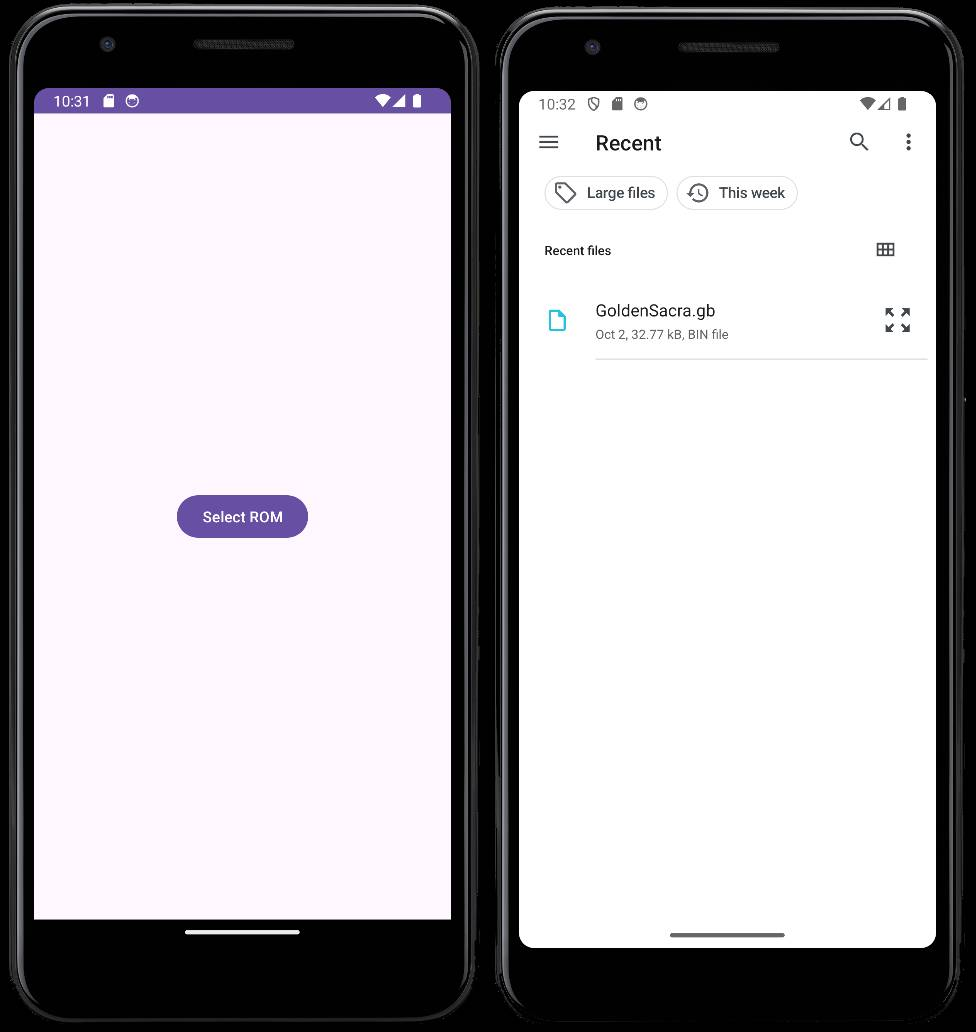
\includegraphics[width=0.4\textwidth]{include/images/openfile.jpg}
\caption{Selección de archivo desde la memoria SD del dispositivo.}
\label{figure:sdopen}
\end{figure}

A continuación, se procede a obtener los bytes del archivo y se envían al módulo de Emulator. En este momento, nos centraremos únicamente en la parte correspondiente a la ROM:

\begin{lstlisting}[language=Kotlin, caption={Carga de ROM y manejo de errores durante el proceso.}, label={code:kotlinloadrom}]
    fun load_rom(romBytes: ByteArray): Boolean{

        try {
            if(romBytes.isNotEmpty()){
                val cartSize = min(romBytes.size, ROM_END - ROM_START + 1)

                for (i in 0 until cartSize) {
                    Memory.write(ROM_START + i, romBytes[i])
                }

                return rom_init(romBytes)
            }
        }catch (ex: Exception){
            println("Error loading ROM: $ex")
        }

        return false
    }
\end{lstlisting}

En la función, se comprueba que los bytes pasados como parámetro no sean nulos. A continuación, se calcula el tamaño total de la ROM para asegurar que no exceda el tamaño máximo permitido (rango de 0x0000 a 0x7FFF). Se escriben todos los bytes en la memoria del emulador, y se invoca la función \textit{rom\_init()} para obtener datos como el título. Si alguna de las operaciones anteriores falla, se devuelve false y la ejecución se detiene.

\begin{lstlisting}[language=Kotlin, caption={Carga de ROM y manejo de errores durante el proceso.}, label={code:kotlinloadromread}]
    enum class CONSOLE_TYPE(val value : Int){
        DMG(0),
        DMG_CGB(0x80),
        CGB(0xC0),
        UNKNOWN(-1);

        companion object {
            fun fromValue(value: Int): CONSOLE_TYPE {
                return entries.find { it.value == value } ?: UNKNOWN
            }
        }
    }
    
    private var bootSection = ByteArray(0xFF)

    private var cartTitle : String      = "Unknown"
    private var licenseCode : String    = "None"
    private var cartType : Int          = -1
    private var romSize : Int           = -1
    private var ramSize : Int           = -1
    private var romVersion : Int        = -1
    private var console: CONSOLE_TYPE   = CONSOLE_TYPE.UNKNOWN

    [...]

    val newLicenseCodes: Map<String, String> = mapOf(
        "00" to "None",
        "01" to "Nintendo R&D1",
        "08" to "Capcom",
        "13" to "Electronic Arts",
        [...]
        "A4" to "Konami (Yu-Gi-Oh!)",
    )

    val oldLicenseCodes : Map<Int, String> = mapOf(
        0x00 to "None",
        0x01 to "Nintendo",
        0x08 to "Capcom",
        0x09 to "HOT-B",
        [...]
        0xFF to "LJN"
    )

    val cartTypes : Map<Int, String> = mapOf(
        0x00 to "ROM ONLY",
        0x01 to "MBC1",
        0x02 to "MBC1+RAM",
        0x03 to "MBC1+RAM+BATTERY",
        0x05 to "MBC2",
        [...]
        0xFF to "HuC1+RAM+BATTERY"
    )

    val ramSizes : Map<Int, Int> = mapOf(
        0x00 to 0, // KiB
        0x01 to 2,
        0x02 to 8,
        0x03 to 32,
        0x04 to 128,
        0x05 to 64
    )

    [...]

    fun convertBytesToString(bytes: ByteArray): String {
        val title = bytes.takeWhile { it != 0.toByte() && it.toInt() in 32..126 } // Filter only ASCII characters
        return String(title.toByteArray(), Charsets.US_ASCII)
    }

    fun rom_init(romBytes: ByteArray): Boolean{

        // Compare Cartridge Header with the Boot fixed one

        // Get header section from the romBytes
        val bootByteArray = Memory.getNintendoLogo()
        val cartByteArray = extractByteArray(romBytes, N_LOGO_START, N_LOGO_END, true) // Nintendo Logo on Cartridge goes from 0x104 to 0x133

        if(memcmp(Memory.getNintendoLogo(), cartByteArray, bootByteArray.size) != 0){
            return false
        }

        cartTitle   = convertBytesToString(extractByteArray(romBytes, TITLE_START, TITLE_END, true))

        licenseCode = if((extractByte(romBytes, OLD_LCNS_CODE).toInt() and 0xFF) == NEW_LICENSE_CODE){
            getNewLicenseNameFromIndex(convertBytesToString(extractByteArray(romBytes, LCNS_CODE_START, LCNS_CODE_END, true)))
        }else{
            getOldLicenseNameFromIndex(extractByte(romBytes, OLD_LCNS_CODE).toInt() and 0xFF)
        }

        cartType    = extractByte(romBytes, CART_TYPE).toInt() and 0xFF
        romSize     = 32 * (1 shl extractByte(romBytes, ROM_SIZE).toInt() and 0xFF) // Value in KiB
        ramSize     = extractByte(romBytes, RAM_SIZE).toInt() and 0xFF
        romVersion  = extractByte(romBytes, ROM_V_NUM).toInt() and 0xFF
        console     = CONSOLE_TYPE.fromValue(extractByte(romBytes, TITLE_END).toInt() and 0xFF)

        println("ROM Loaded Successfully!")

        bootSection = extractByteArray(romBytes, 0x00, 0xFF, true) // Save portion of code where the boot is going to load

        return true
    }
\end{lstlisting}

Desglosemos el código:

\begin{enumerate}
    \item Se compara el logotipo de Nintendo almacenado en el módulo de memoria con el presente en el cartucho. Si no coinciden, se procede a finalizar la ejecución del programa.
    \item Se obtienen los bytes correspondientes al título del juego y se convierten a una cadena de texto utilizando el conjunto de caracteres ASCII. Dado que la longitud del título depende de la versión del cartucho, se detendrá la lectura al encontrar el primer valor 0x00.
    \item Se extrae el código de licencia. Primero, se verifica si el valor antiguo contiene 0x33 para utilizar los nuevos códigos de licencia. De lo contrario, se empleará el listado antiguo. Ambos listados pueden definirse mediante un par de mapas (\textit{Maps}) para acceder rápidamente al valor correspondiente según el código obtenido.
    \item A continuación, se extraen de manera directa los valores correspondientes al tipo de cartucho, tamaño de la ROM/RAM, versión de la ROM y el tipo de mapper.
    \item Se realiza una copia de la región 0x0000-0x00FF del cartucho. La Game Boy "oculta" esta porción de código hasta que la secuencia de arranque ha finalizado.
\end{enumerate}

Aquí los resultados obtenidos con la carga de las ROMS \textit{Super Marioland}, \textit{Pokémon Azul} y \textit{Harry Potter y la Piedra Filosofal}:

\begin{lstlisting}[language=Consola, caption={Valores obtenidos tras la carga de ROM.}, label={code:romresults}]
--- Super Marioland
Cart Title: SUPER MARIOLAND
License: Nintendo
Cart Type: MBC1
ROM Size: 64
ROM Version Number: 0
RAM Size: 0
Console Type: DMG

--- Pokemon Azul
Cart Title: POKEMON BLUE
License: Nintendo R&D1
Cart Type: MBC5+RAM+BATTERY
ROM Size: 1024
ROM Version Number: 0
RAM Size: 3
Console Type: DMG

--- Harry Potter y la Piedra Filosofal
Cart Title: HARRYPOTTERBHVE
License: EA (Electronic Arts)
Cart Type: MBC5+RAM+BATTERY
ROM Size: 4096
ROM Version Number: 0
RAM Size: 2
Console Type: CGB
\end{lstlisting}

Además, se puede observar que la ROM se ha cargado correctamente en nuestra memoria virtual. En el caso de \textit{Harry Potter} y la piedra filosofal, los siguientes bytes son visibles en la región 0x0000-0x015F:

\begin{lstlisting}[language=Consola, caption={Visualización de la ROM cargada en la memoria virtual.}, label={code:rommemloaded}]
0000: E1 CD 9D 31 E9 87 87 87 85 6F 3E 00 8C 67 7E C9  | ...1.....o>..g~.
0010: 7A BC C0 7B BD C9 FF FF 3E 01 E0 A6 C9 FF FF FF  | z..{....>.......
0020: AF E0 A6 3E 02 E0 A8 C9 7C E0 51 7D E0 52 7A E0  | ...>....|.Q}.Rz.
0030: 53 7B E0 54 79 E0 55 C9 40 F5 D1 7B EA BA CD C9  | S{.Ty.U.@..{....
0040: C3 80 36 FF FF FF FF FF C3 CE C0 C3 AC 23 FF FF  | ..6..........#..
0050: FB C3 AC 39 FF FF FF FF C3 A3 38 FF FF FF FF FF  | ...9......8.....
0060: D9 D7 38 04 D5 54 5D E1 CB 2A CB 1B CB 2A CB 1B  | ..8..T]..*...*..
0070: CB 2A CB 1B 19 19 19 C9 CB 7C C8 F5 7D 2F C6 01  | .*.......|..}/..
0080: 6F 7C 2F CE 00 67 F1 C9 F5 79 2F C6 01 4F 78 2F  | o|/..g...y/..Ox/
0090: CE 00 47 F1 C9 CB 7A C8 F5 7B 2F C6 01 5F 7A 2F  | ..G...z..{/.._z/
00A0: CE 00 57 F1 C9 C5 06 08 AF 87 CB 15 30 04 84 30  | ..W.........0..0
00B0: 01 2C 05 20 F4 65 6F C1 C9 AF B5 20 03 65 37 C9  | .,. .eo.... .e7.
00C0: C5 D5 06 08 4D 2E 00 CB 14 CB 15 5D 7D 91 6F 3F  | ....M......]}.o?
00D0: 38 01 6B 05 20 F1 CB 14 B7 D1 C1 C9 C5 4D 44 3E  | 8.k. ........MD>
00E0: 0F 21 00 00 CB 23 CB 12 30 01 09 29 3D 20 F5 CB  | .!...#..0..)= ..
00F0: 7A 28 01 09 C1 C9 19 3E 02 EA 00 20 5E 23 56 C9  | z(.....>... ^#V.
0100: 00 C3 50 01 CE ED 66 66 CC 0D 00 0B 03 73 00 83  | ..P...ff.....s..
0110: 00 0C 00 0D 00 08 11 1F 88 89 00 0E DC CC 6E E6  | ..............n.
0120: DD DD D9 99 BB BB 67 63 6E 0E EC CC DD DC 99 9F  | ......gcn.......
0130: BB B9 33 3E 48 41 52 52 59 50 4F 54 54 45 52 42  | ..3>HARRYPOTTERB
0140: 48 56 45 C0 36 39 00 1B 07 02 01 33 00 D7 B4 78  | HVE.69.....3...x
0150: A7 FE 11 3E 00 20 01 3C E0 EF 31 FF CF F0 EF B7  | ...>. .<..1.....
\end{lstlisting}

\subsection{Lectura/Escritura en ROM}


\cleardoublepage